\chapter{Discrete modeling of the dynamics on the spatially uniform membrane}

\label{Monte_Carlo_model_description}

\section{Monte-Carlo automaton description}

The work presented in this chapter has been published in the paper of Kiselev et al. \cite{Kiselev2011} and has been done by me.

To begin a computational investigation of the lateral dynamics of lipids and proteins on the cell membrane, I develop a kinetic Monte-Carlo simulation model (or kinetic Monte-Carlo automaton, MCA hereafter) \cite{Rubinstein2008}, which faithfully describes the diffusion of lipid species and proteins on the cellular membrane under the action of random thermal noise (Brownian motion) and electrostatic forces.

Generally, any Monte-Carlo simulation procedure is based on a random sampling, which is repeatedly used to decide whether to accept or reject any change in the system configuration. In the MCA under consideration, in order to make this decision, I use Metropolis-Hastings algorithm \cite{Metropolis1953}. Metropolis-Hastings algorithm requires calculation of an expected energy cost ($\Delta E$) caused by the change. Depending on the energy cost the change can be either accepted or rejected. If $\Delta E < 0$ the change brings the system to a state of lower energy, thus it is always accepted (according to the second law of thermodynamics). If $\Delta E > 0$ the change is accepted with the probability $P=\exp(-\Delta E/k_BT)$, where $k_B$ is Botzmann constant and $T$ is the temperature of the system. To accept the change with the probability $P$, a random number $R$ ($R$ $\in$ [0:1]) is generated and compared with $P$. If $P > R$ then the change is accepted, otherwise it is rejected.

Due to the membrane topology, the MCA is constructed in a two-dimensional space (2D) and consists of two parallel hexagonal lattices, separated by a small distance and embedded into the cytoplasmic solution. The first hexagonal lattice represents the inner leaflet of the cell membrane, while the second one represents the plane of the protein diffusion. In the simulations of the MCA I consider a protein with a PD and a single lipid modification (section \ref{adsorption_introduction0}).

Every node of the lipid lattice is occupied by a lipid head group. Since the membrane is not static and lipid head groups are able to move out of the main leaflet plane, I assume that in the MCA the lipid head groups are always surrounded by cytoplasmic ions (alternatively, the cytoplasmic ions can freely penetrate the layer). In this case the lipid head groups in the MCA are always equilibrated with the cytoplasmic ions, due to their high mobility.

To concentrate on electrostatic properties of the protein membrane dynamics in the protein lattice, instead of a whole protein, I consider the diffusion of its PD. Particularly, I simplify the PD by an oligopeptide consisting of only positively charged residues. Similar to the approach described in \cite{Denisov1998} I choose pentalysine Lys-5 with five basic residues and, consequently, with the charge +5, as such an oligopeptide. In the MCA this peptide always diffuses in the lattice overlying the lipid lattice.

The lipids and the peptide diffuse in their lattices under the action of random thermal noise (Brownian motion) and electrostatic forces. The size of the membrane lattice $L$ is chosen to be less then 100 nm, which allows to simulate the evolution of the membrane in a computationally efficient way. However, since the numerical complexity of the simulations is proportional to $L^2$, further increase in the lattice dimension reduces the effectiveness of the algorithm. Thus, simulations of the system with larger $L$ have to be performed in the context of a different modeling framework (see chapter \ref{continuous_model_description}). The total observation time $\tau_0$ is chosen to be less than 0.01 s. Experimental data suggests that the characteristic membrane association time of proteins with a PD and a single lipid modification is on the order of seconds \cite{Fivaz2003}. Therefore, since the evolution time in the MCA $\tau_0\ll1$ s, I assume that the protein is always bound to the membrane and does not dissociate from it during the simulations.

\subsection{Lipid lattice structure}
\label{model_description}

To define the unit size ($d$) of the lipid lattice I use an experimentally measured (at 30$^\circ$ C) value of the average lipid head group area $A_L \sim$ 0.6 nm$^2$ \cite{Petrache2000}. Using simple geometrical calculations one can derive the following (see Fig. \ref{fig:lipid_area} for the details):

\begin{figure}[!ht]
%\centering
%\scalebox{1.0}[1.0]
\begin{center}
  \includegraphics[scale=1.2]{../figures/lipid_area.pdf}
\end{center}
 \caption[Schematic representation of the membrane lattice]{Schematic representation of the membrane lattice. Lipids are shown as grey circles; a hexagon around any lipid has an area $A_L$; $d'$ is the size of the hexagon side; $d$ is the lattice unit size (the distance between two neighboring lipid head groups); $S$ is the area of the equilateral triangle with the side $d'$.}
\label{fig:lipid_area}
\end{figure}


\begin{equation}
 A_L = 6 S
\end{equation}
\begin{equation}
 S = \frac{\sqrt{3}(d')^2}{4}
\end{equation}
\begin{equation}
 d' = \frac{d}{\sqrt{3}}
\end{equation}

Solution of these equations provides an analytical expression for $d$:

\begin{equation}
 d = \sqrt{\frac{2A_L}{\sqrt{3}}}
\end{equation}

For A$_L \sim$ 0.6 nm$^2$ the distance $d\simeq$ 0.8 nm. This value of $d$ is used everywhere throughout the simulations. The lipid lattice nodes are populated with 3 types of lipids described in the subsection \ref{phospholipids}: neutral PC lipids (with charge 0) monovalent negatively charged PA or PS lipids (with charge -1, referred in the text as PS), and multivalent negatively charged PIP$_2$ lipids (with charge -4).

\subsection{PD structure}

\label{polybasic_domain_structure}

Previously reported structure of Lys-5 peptide \cite{Ben-Tal1996}, which is chosen as a prototype of a protein with the PD, suggests that the positively charged residues of the peptide can be projected onto the membrane hexagonal lattice with minimal deformations, so that the residues approximately match with some of the lipid nodes (see Fig. \ref{fig:lys5_structure}).
\begin{figure}[!ht]
%\centering
%\scalebox{1.0}[1.0]
\begin{center}
  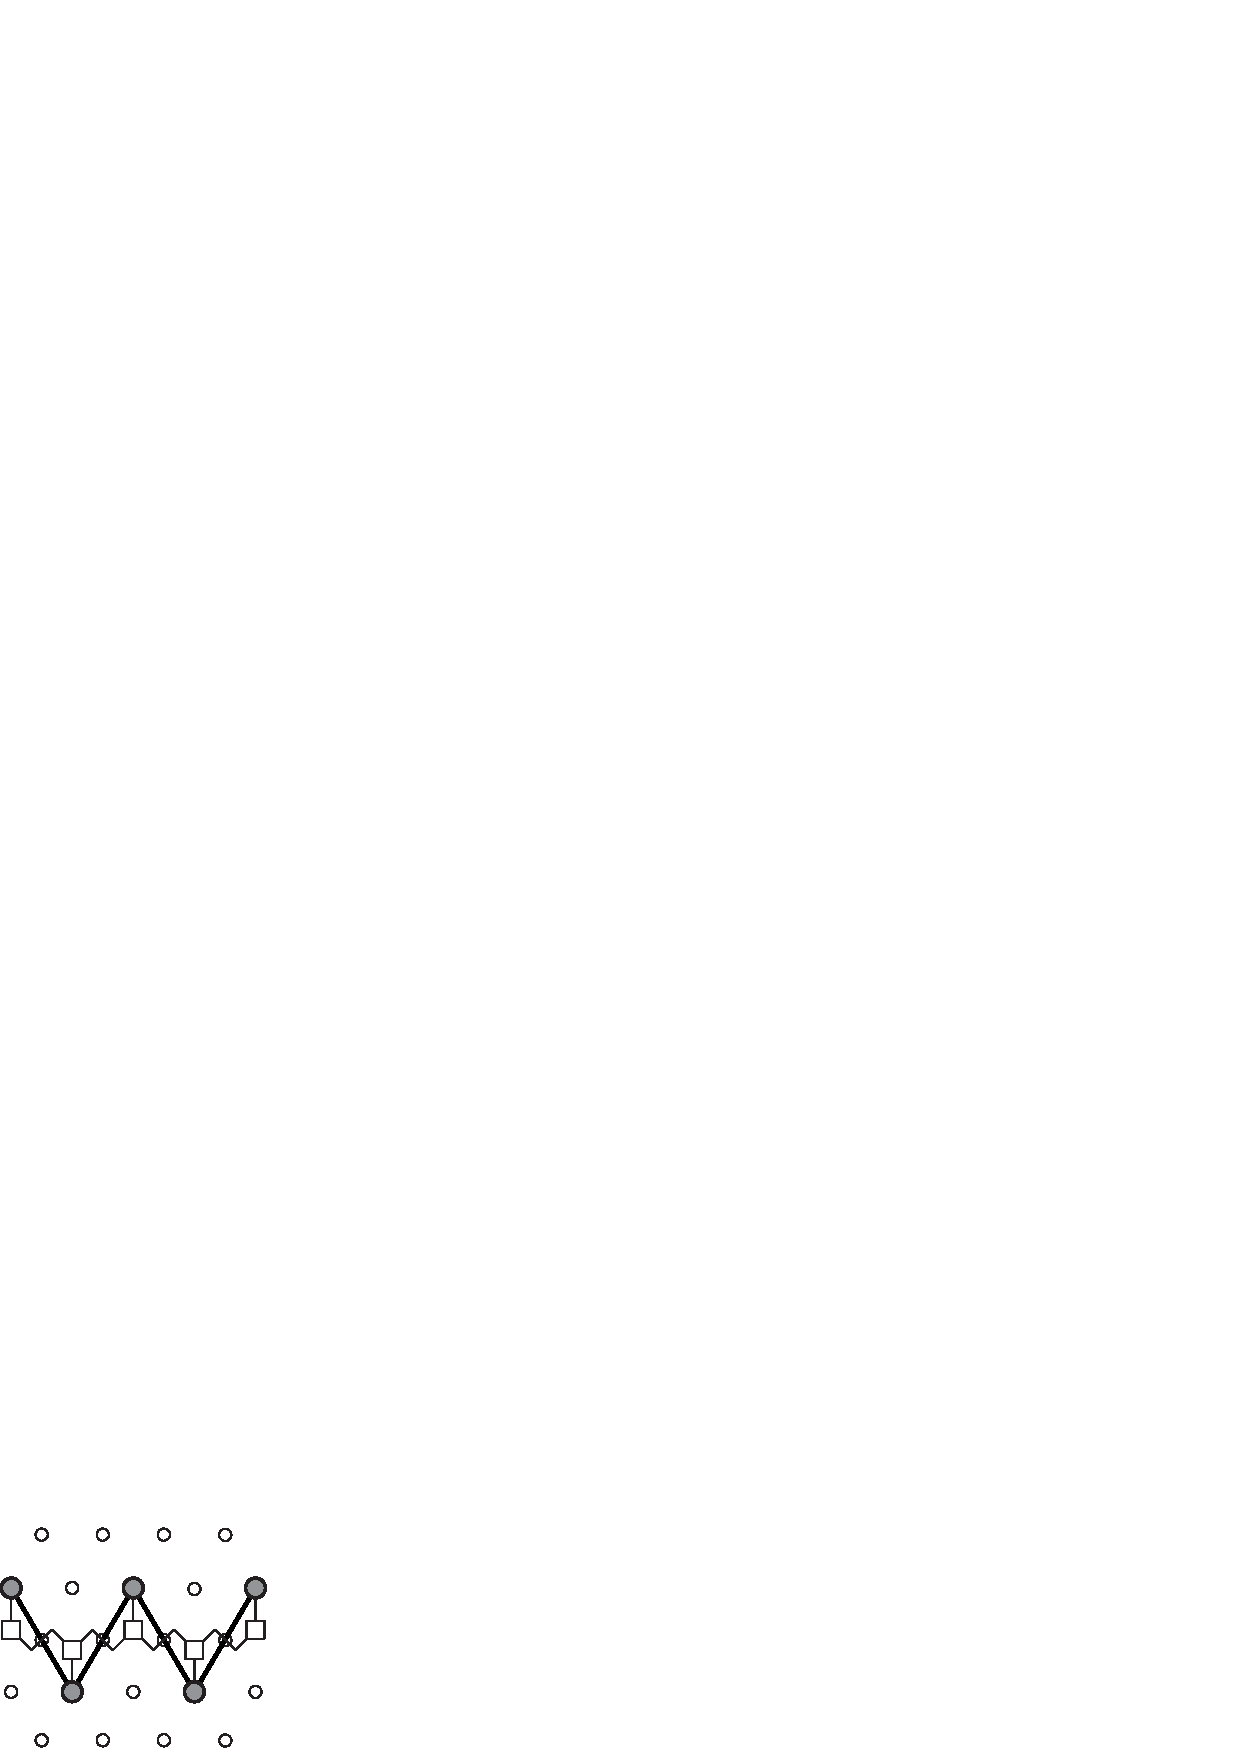
\includegraphics[scale=1.5]{../figures/lys5_structure.pdf}
\end{center}
 \caption[Projection of Lys-5 peptide backbone on the lipid lattice.]{Projection of Lys-5 peptide backbone (from \cite{Kiselev2011}) on the lipid lattice (open circles). $\alpha$-Carbons are denoted by open squares, and positively charged side chains are indicated by solid circles.}
\label{fig:lys5_structure}
\end{figure}
Utilizing this approximation I use a W-shaped ball-and-stick structure as a model structure of Lys-5 in the MCA. Due to the matching between the two model lattices, the peptide lattice is chosen to be topologically identical to the lipid one. Thus, during one simulation step, the distance, by which the peptide can be displaced, equals the lipid lattice unit size $d$. I assume that the peptide and lipid lattices are separated by D$_{H_2O}$ = 0.28 nm (the diameter of one water molecule). This distance is chosen based on the previous studies \cite{Murray1997,Murray1999}, suggesting that it is optimal for a balance between the Coulombic attraction and desolvation penalties. However, \emph{in vivo}, due to the vertical mobility of the lipid head groups in the membrane plane, this distance can presumably increase, allowing the cytoplasmic mobile ions to freely penetrate and equilibrate in the peptide-membrane space. I use this hypothesis in the MCA, assuming that the peptide-membrane space is always occupied by cytoplasmic mobile ions.

\subsection{Calculation of the interaction energies}

\label{interaction_energies}

I assume that all lipids and Lys-5 residues are point charges that interact only electrostatically and can populate only lattice discrete nodes. The electrostatic potential of the interaction is chosen to be the screened Coulomb potential (also known as Yukawa potential):
\begin{equation}
\label{yukawa_potential}
 V(r) = \frac{q_1q_2}{4\pi\varepsilon\varepsilon_0}\frac{e^{-r/\lambda}}{r}
\end{equation}
where $q_1$ and $q_2$ are the values of the interacting charges, $r$ is the distance between them, $\varepsilon$=80 is the dielectric constant of water, $\varepsilon_0$ is the vacuum permittivity and $\lambda$ is the Debye length. The Debye length for an ionic solution is a function of the temperature and the ionic strength $I$:
\begin{equation}
 \lambda = \sqrt{\frac{\varepsilon\varepsilon_0k_BT}{2N_Ae^2I}}
\end{equation}
where $N_A$ is Avogrado's number.

The ionic strength is defined by the following equation:
\begin{equation}
 I=\frac{1}{2}\sum_{i=1}^{n}c_iz_i^2
\end{equation}
Where c$_i$ is the molar concentration of ion $i$ in the cytoplasm, z$_i$ is its charge. The cytoplasmic liquid is usually considered as a 0.1 M 1:1 electrolyte \cite{Khelashvili2008,May2000}. Thus, I use the value of the Debye length, calculated for this solution, in the majority of the simulations: $\lambda$ = 1 nm. Since mobile ions are equilibrated with both the lipids and the peptide the Debye length is assumed to be constant in every point of the MCA system.

According to eq. \eqref{yukawa_potential} the strongest interactions in the membrane lattice correspond to the minimal possible distance between any two lipids $d = 0.8$ nm. Similarly, the strongest interaction between a peptide residue and a lipid occurs when the lipid is located directly underneath the peptide residue, so that the distance between them is minimal (D$_{H_2O}$ = 0.28 nm, see subsection \ref{polybasic_domain_structure}). The values of the maximal interaction energies between any two particles of the MCA can be calculated from the eq. \eqref{yukawa_potential}: E$_\text{PS-PS}$ $\simeq$ 0.4 k$_B$T, E$_\text{PS-PIP$_2$}$ $\simeq$ 1.6 k$_B$T, E$_\text{PIP$_2$-PIP$_2$}$ $\simeq$ 6.4 k$_B$T, E$_\text{Lys-PS}$ $\simeq$ --1.9 k$_B$T and E$_\text{Lys-PIP$_2$}$ $\simeq$ --7.6 k$_B$T.

To illustrate how the interaction energy depends on the distance, I calculate it for a general case of two lipids interacting at different distances (Fig. \ref{fig:yukawa_lipid_energies}).
\begin{figure}[!ht]
%\centering
%\scalebox{1.0}[1.0]
\begin{center}
  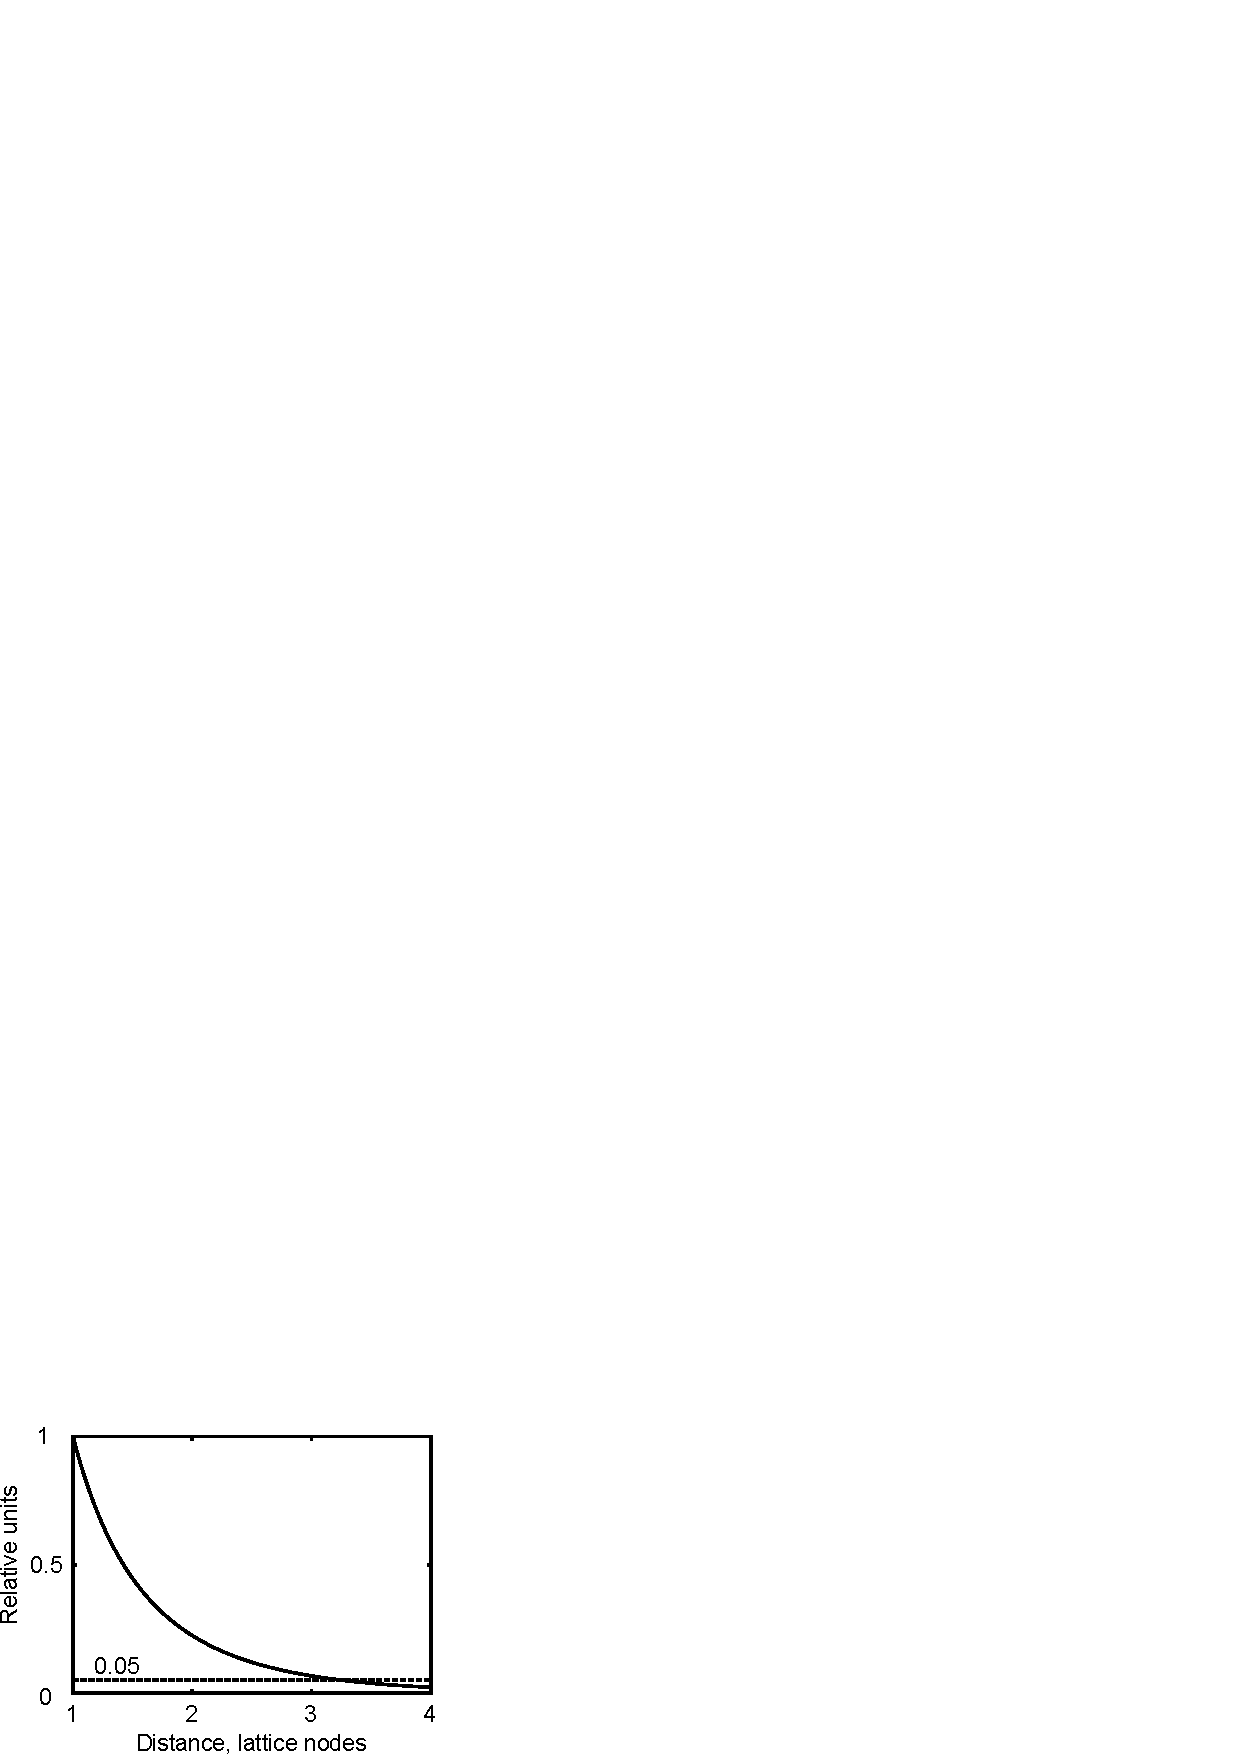
\includegraphics[scale=1.2]{../figures/yukawa_lipid_energies1.pdf}
\end{center}
 \caption[Dependence of the interaction energy of lipids on distance]{Dependence of the interaction energy of lipids on distance. The interaction potential, $V(q_1,q_2,x)$ between any two lipids $q_1$ and $q_2$ at the distance $x$ lattice nodes, normalized by its maximal value $V(q_1,q_2,1)$ at the distance 1 lattice node is shown as a solid black line. Level of the energy corresponding to the 5\% of the maximal value is shown as a black dashed line.}
\label{fig:yukawa_lipid_energies}
\end{figure}

\subsection{Calculation of $\Delta E$ induced by a system change}

\label{delta_energy_calculation}

Lipid movements are implemented by means of Kawasaki algorithm \cite{Kawasaki1972}. This algorithm represents the diffusion of particles in a compact media, where the particles swap positions during their movements. Each lipid in the model during any movement swaps its position with a randomly chosen neighboring lipid. The energy cost induced by this swap ($\Delta E$) is required to be computed by the MC algorithm. Since, during the interchange of the two lipids, the rest of the system remains static, the energy cost can be computed by taking into account only interactions of the moving lipids with the rest of the membrane (instead of computing the interactions of all charged particles in the system with each other). Moreover, Fig. \ref{fig:yukawa_lipid_energies} shows that at the distance of $>$3 lattice nodes between any two lipids, the energy of interaction of these lipids decreases to less than 5$\%$ of the maximal energy. Thus, one can define a 3-node hexagonal neighborhood of the moving lipids, where the energy cost induced by the movement is computed, neglecting the contributions of the lipids lying outside the neighborhood. This is equivalent to cutting off the potential in eq. \eqref{yukawa_potential} above $\sim$3 Debye length. The lipid neighborhood is shown schematically in Fig. \ref{fig:lipid_neighborhood}. I use this neighborhood in calculations of $\Delta E$ induced by the lipid movements.

\begin{figure}[!ht]
%\centering
%\scalebox{1.0}[1.0]
\begin{center}
  \includegraphics[scale=1.8]{../figures/lipid_neighborhood.pdf}
\end{center}
 \caption[The neighborhood used to calculate $\Delta E$ of the lipid movement]{The neighborhood (from \cite{Kiselev2011}) used to calculate $\Delta E$ of the lipid movement is indicated by the solid line. Charged lipids are shown as solid circles.}
\label{fig:lipid_neighborhood}
\end{figure}

In simulations the peptide as a complex rigid structure undergoes two types of movements -- translational and rotational. Translational movement is implemented as a displacement of the whole peptide (all five residues) in one out of six directions, chosen at random. Importantly, if the mobility of the peptide is lower than that of the membrane lipids, the lipids will perform a fast demixing, resulting in binding of a large number of the negatively charged lipids to the peptide residues. Lys-5 at relevant biological conditions (25$\%$ PS, 75$\%$ PC) accumulates at its residues about 4 negatively charged PS lipids (see section \ref{lipid_demixing}). If the peptide moved independently from these lipids it would require an energy cost $\Delta$E of about +7.6 k$_B$T. The probability of such a movement to be accepted is $\exp(-\Delta E/k_B T) \approx 10^{-3}$, resulting in effective immobilization of the peptide. In ternary membranes, containing multivalent PIP$_2$ the energy cost would be even higher and the peptide immobilization would be stronger. The resulting stalemate in the peptide diffusion was previously described in \cite{Khelashvili2008}. However, this phenomenon is known and is called a kinetic trapping. It is usually caused by strong short-range particle interactions. To overcome kinetic trapping, Whitelam and Geissler \cite{Whitelam2007} proposed to introduce collective moves to the system. Thus, instead of the single peptide, the total complex, consisting of the peptide and lipids bound to it, undergoes the lateral diffusion. In this case the energy cost corresponding to the peptide movement does not include the energy of breaking of the peptide-lipid binding. I use this approximation in the MCA. Thus, the peptide movement in the model is always accompanied by a swapping of lipids directly bound to peptide residues with neighboring lipids. The energy cost of the resulting collective movement is then computed (in a similar way, described for the lipids above) within an asymmetrical neighborhood extended in the direction of the proposed movement (Fig. \ref{fig:peptide_neighborhood}).
\begin{figure}[!ht]
%\centering
%\scalebox{1.0}[1.0]
\begin{center}
  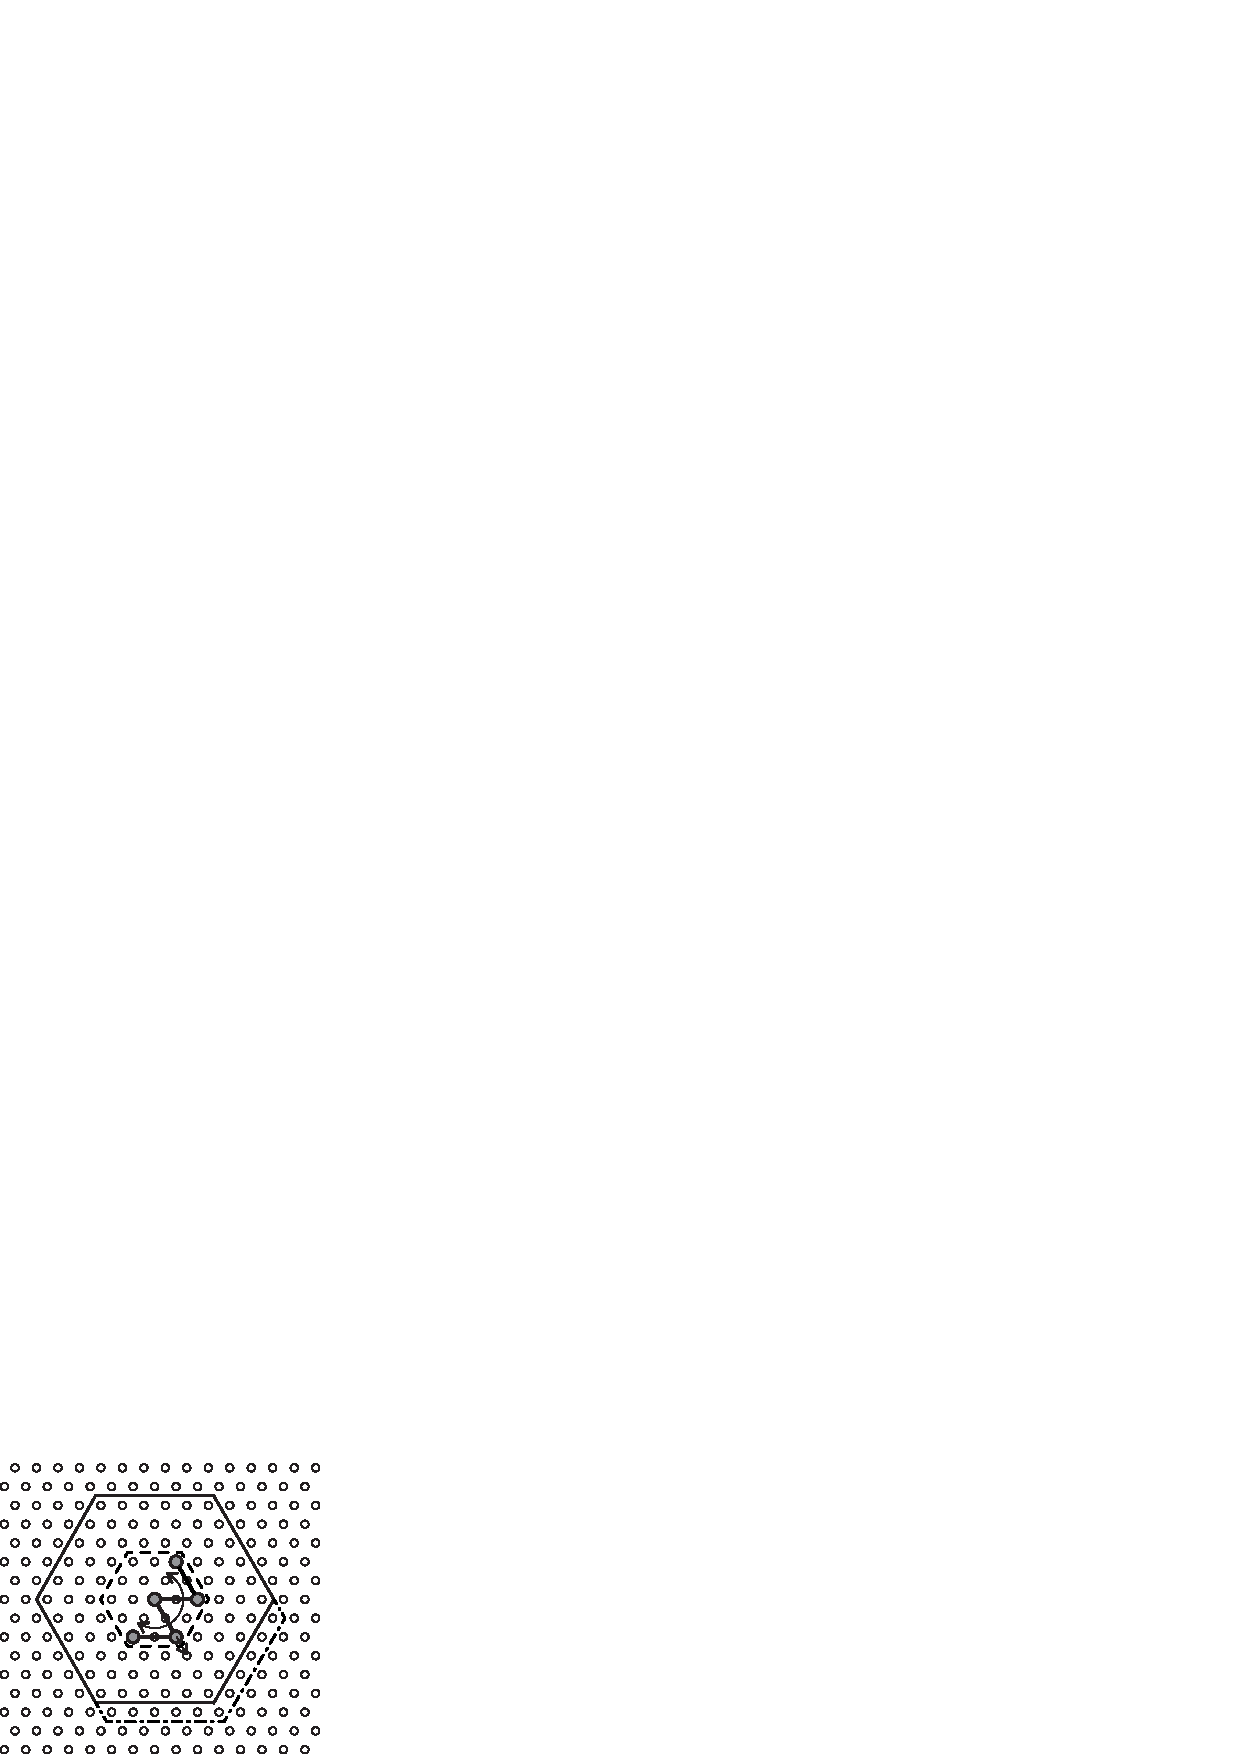
\includegraphics[scale=1.8]{../figures/peptide_neighborhood.pdf}
\end{center}
 \caption[The neighborhoods used to calculate $\Delta E$ of the peptide translational and rotational movements]{The neighborhoods (from \cite{Kiselev2011}) used to calculate $\Delta E$ of the peptide translational and rotational movements are shown by dash-dotted and solid lines, respectively. Lipids enclosed within the hexagon shown by the dashed line rotate together with the peptide.}
\label{fig:peptide_neighborhood}
\end{figure}

Since the peptide structure is projected onto the hexagonal lattice, I choose a central peptide residue as the best approximation of the center of mass of the peptide. At every simulation step the peptide undergoes rotation around the central node by $\pm$60$^\circ$, where the sign is chosen randomly. To avoid kinetic trapping in the case of the peptide rotation, all lipids located in the peptide hexagon envelope (Fig. \ref{fig:peptide_neighborhood}) rotate together with the peptide. The energy cost related to the rotation is calculated in the symmetric neighborhood area (Fig. \ref{fig:peptide_neighborhood}). Interestingly, the necessity of the peptide rotation becomes clear already at a small fraction of PIP$_2$ in the membrane, as the peptide accumulates a large negative charge and starts repelling membrane charged lipids. Due to the intrinsic asymmetry of the peptide structure (3 residues on the one side against 2 residues on the other side), its interaction with the membrane lipids is not symmetric. This asymmetry produces an artificial net force acting on the peptide, making its motion biased. Thus, although the rotation mechanism described above does not faithfully represent the corresponding \emph{in vivo} or \emph{in vitro} rotation of a real protein with a PD, it is required for the symmetry of the peptide diffusion. 

Note that, since the rotation is discrete, during one rotational step all peptide residues and some of the lipids in the peptide hexagon envelope are displaced by 2 lattice nodes with respect to their initial positions, i.e. their movements are non-local (the displacement is more than 1 node). However, this rotational movement is only important for the interactions of all particles in the peptide hexagon envelope with the lipids that are in the vicinity of the envelope (the peptide nodes and lipids in the hexagon envelope do not change their positions with respect to it). Since the concentration of lipids around the envelope is almost undisturbed (see Fig. \ref{fig:lipid_demixing_profiles}), the rotational move does not significantly change the system configuration. Therefore, I neglect the possible non-Brownian effect that can be caused by the non-local moves during the discrete peptide rotation.

The energy cost of the rotational movement is computed (in a similar way, described for the translational peptide movement above) within an symmetrical hexagonal neighborhood represented in Fig. \ref{fig:peptide_neighborhood} by a solid line.


\subsection{MCA implementation}

\label{model_implementation}

Periodic boundary conditions are imposed on the dynamics of both the lipids and the peptide. One complete time step of the simulations consists of the following:
\begin{enumerate}
 \item All charged lipids attempt to move by one node in the membrane lattice, including those directly underneath the peptide nodes. This mechanism is implemented using the following procedure. Starting from a randomly chosen corner of the membrane lattice and moving in a typewriter manner, all charged lipids are picked and are forced to move;
 \item \label{2} The peptide tries to move by one node in the peptide lattice;
 \item \label{3} The peptide attempts to rotate around its central node;
\end{enumerate}

All simulations are performed using custom written C code on a multiprocessor Dell Precision T7400 workstation.

\subsection{Testing and calibration of the MCA}

\label{testing_calibration_MCA}

The MCA described above has been extensively tested and validated to ensure that it adequately represents the dynamics of the system at hand. The results are obtained from averaging over several thousand independent realizations. The averaged values of horizontal and vertical displacements $\langle x\rangle$, $\langle y\rangle$ and the mean squared displacement $\langle r^2\rangle$ are computed for the lipid species. As expected $\langle x\rangle$ and $\langle y\rangle$ are close to and fluctuate around 0 and $\langle r^2\rangle$ is directly proportional to the time of the simulation ($\langle r^2\rangle\sim t$). Thus, lipids undergo Brownian diffusion without drift. The rejection rate of lipid dynamics is also checked for the relevant biological conditions (25$\%$ PS and 75$\%$ PC) and appeared to be negligible suggesting that lipid moves are mostly accepted. The peptide dynamics has been checked in the same way and has been also proved to be Brownian.

The fact that lipids undergo Brownian diffusion allows one to naturally calibrate the model. Having a fixed value of lattice spatial resolution I computed the diffusion coefficient of lipids in the uncharged membrane from the equation of Brownian law:

\begin{equation}
 \langle r^2\rangle = 4Dt
\end{equation}

The obtained value is D = 0.3 $d^2/\Delta t$, where $d$ is the inter-lipid distance and $\Delta t$ is the time of one iteration. Remembering that the distance between two neighboring lipids $d$ = 0.8  nm = $8\cdotp10^{-4}$ $\mu$m, the diffusion coefficient can be rewritten in different units: $D = 3.2\cdotp10^{-7}$ $\mu$m$^2$/$\Delta t$. Assuming that the typical \emph{in vivo} lipid diffusion coefficient is $D_L$ = 1 $\mu\text{m}^2/\text{s}$, the ``real'' time of 1 iteration can be calculated as: $\Delta t$ = 0.32 $\mu$s. Since the rejection rate of lipid dynamics for relevant biological conditions is negligibly low no further rescaling of the automaton by the acceptance rate is needed (as suggested in \cite{Sanz2010}).

As described in subsection \ref{model_implementation} the frequencies of peptide and lipid translational moves are equal. This condition automatically defines the maximal achievable diffusion coefficient of the peptide $D_0$ (when all peptide moves are accepted, i.e. when the system is neutral). As in the lipid case, a suitable experimental value of $D_0$ can be used to convert the obtained valued of the peptide diffusion coefficient into dimensional units. To make the peptide diffusion coefficient smaller than $D_0$, the frequency of the peptide moves can be manually reduced to the necessary value, correspondingly slowing down the peptide diffusion.

\subsection{Limitations of the MCA}

It is important to discuss the limitations of the constructed MCA:

\begin{enumerate}
 \item The model neglects possible hydrodynamic effects beyond the viscous drag. The viscous drag is naturally determined by scaling the model using experimentally measured lipid and protein diffusion coefficients.
 \item Although Yukawa potential \eqref{yukawa_potential} faithfully describes interaction of ions in the electrolyte solution, the model could be improved by using a more detailed Poisson-Boltzmann approach.
 \item Ideally, multi-scale or all-atom simulations can be used to better describe the membrane dynamics. However, all of these methods would greatly increase the numerical complexity and, therefore, would require to reduce the size of the system, making it impossible to obtain the effects described in this thesis.
\end{enumerate}

Although these limitations are important, I expect that the simulation results, obtained in the MCA, faithfully describe the membrane dynamics of lipids and proteins.


\section{Results}

This section summarizes the results obtained in the MCA for the case of the uniform lipid distributions in the membrane. All membrane concentrations mentioned in this chapter are fixed, constant and uniform.

\subsection{Lipid sequestration and demixing}

\label{lipid_demixing}

First, I qualitatively measure the electrostatic interactions between the protein PD and the membrane anionic lipids. Since the PD in the MCA is represented by Lys-5 peptide, which structure can be projected to the lipid lattice, there are always 5 nodes in the membrane lattice that are the closest to the Lys-5 basic residues. The interaction of these residues with underlying lipids is the strongest compared to the interactions with other lipids. Thus, the underlying lipids locate in the most preferable positions for interactions. Fig. \ref{fig:occupation_probabilities}, A shows the steady state probability of these positions being occupied by PS in the case of a binary PC/PS membrane. In the physiological range of PS
\begin{figure}[!ht]
%\centering
%\scalebox{1.0}[1.0]
\begin{center}
  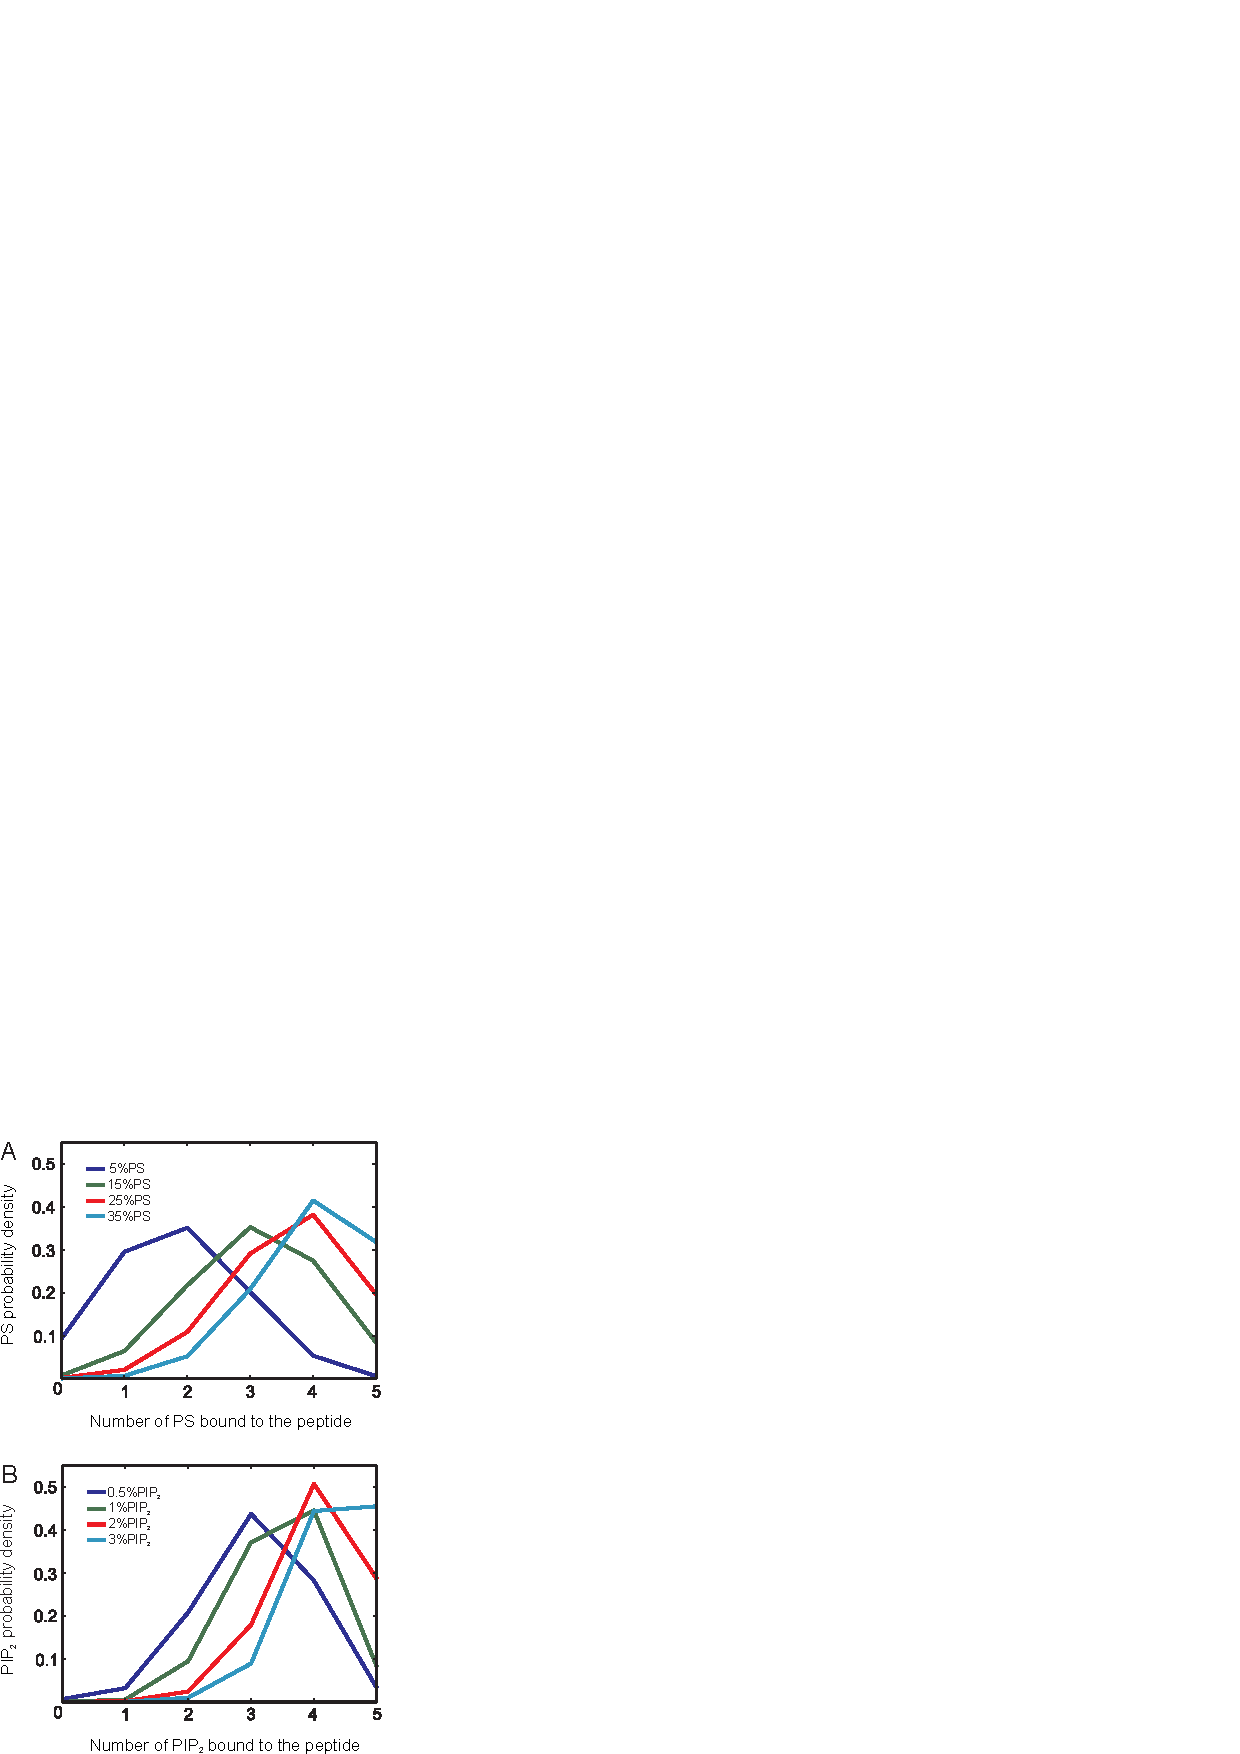
\includegraphics[scale=1.3]{../figures/occupation_probabilities.pdf}
\end{center}
 \caption[Probability density functions of lipid association for PS and PIP$_2$]{Probability density functions of lipid association (from \cite{Kiselev2011}) for PS (A) and PIP$_2$ (B). For all plots in B, the PS fraction is 25\%.}
\label{fig:occupation_probabilities}
\end{figure}
concentrations (15-25\%) the peptide basic residues are never fully occupied by monovalent PS lipids. Even at unrealistically high PS concentrations, the total charge of the peptide (the actual charge of the peptide plus the sum of the charges of all lipids in the underlying positions) remains positive (Fig. \ref{fig:total_peptide_charge}).
The situation significantly changes in the case of a ternary PC/PS/PIP$_2$ membrane (Fig. \ref{fig:occupation_probabilities}, B). Even at a small concentration (0.5\%) about three multivalent PIP$_2$ lipids are associated with the peptide, making the total charge of the peptide strongly negative, -7 (Fig. \ref{fig:total_peptide_charge}).

I also computed the same occupation probabilities for Lys-6 and Lys-7. The data (not presented here) shows that on binary PC/PS membrane the occupations of all three peptides per one peptide residue are almost identical. This suggests that the peptide residues in the constructed MCA interact with anionic membrane lipids independently of each other.
\begin{figure}[!ht]
%\centering
%\scalebox{1.0}[1.0]
\begin{center}
  \includegraphics[scale=1.4]{../figures/ps_pip_competition.pdf}
\end{center}
 \caption[Average numbers of PS and PIP$_2$ molecules associated with the peptide]{Average numbers of PS and PIP$_2$ molecules (from \cite{Kiselev2011}) associated with the peptide at varying lipid concentrations.}
\label{fig:ps_pip_competition}
\end{figure}
\begin{figure}[!ht]
%\centering
%\scalebox{1.0}[1.0]
\begin{center}
  \includegraphics[scale=1.4]{../figures/total_peptide_charge.pdf}
\end{center}
 \caption[Total peptide charge]{Total peptide charge (from \cite{Kiselev2011}) -- the charge of the peptide together with associated lipids.}
\label{fig:total_peptide_charge}
\end{figure}
Thus, in the case of binary PC/PS membrane, the results above can be also applicable to a peptide with a variable length.

Second, Fig. \ref{fig:ps_pip_competition} shows that monovalent PS and multivalent PIP$_2$ lipids effectively compete with each other for the preferable underlying positions underneath the peptide. At concentrations higher than 0.5\% PIP$_2$ lipids practically displace all monovalent PS lipids from the peptide residues.

\begin{figure}[!ht]
%\centering
%\scalebox{1.0}[1.0]
\begin{center}
  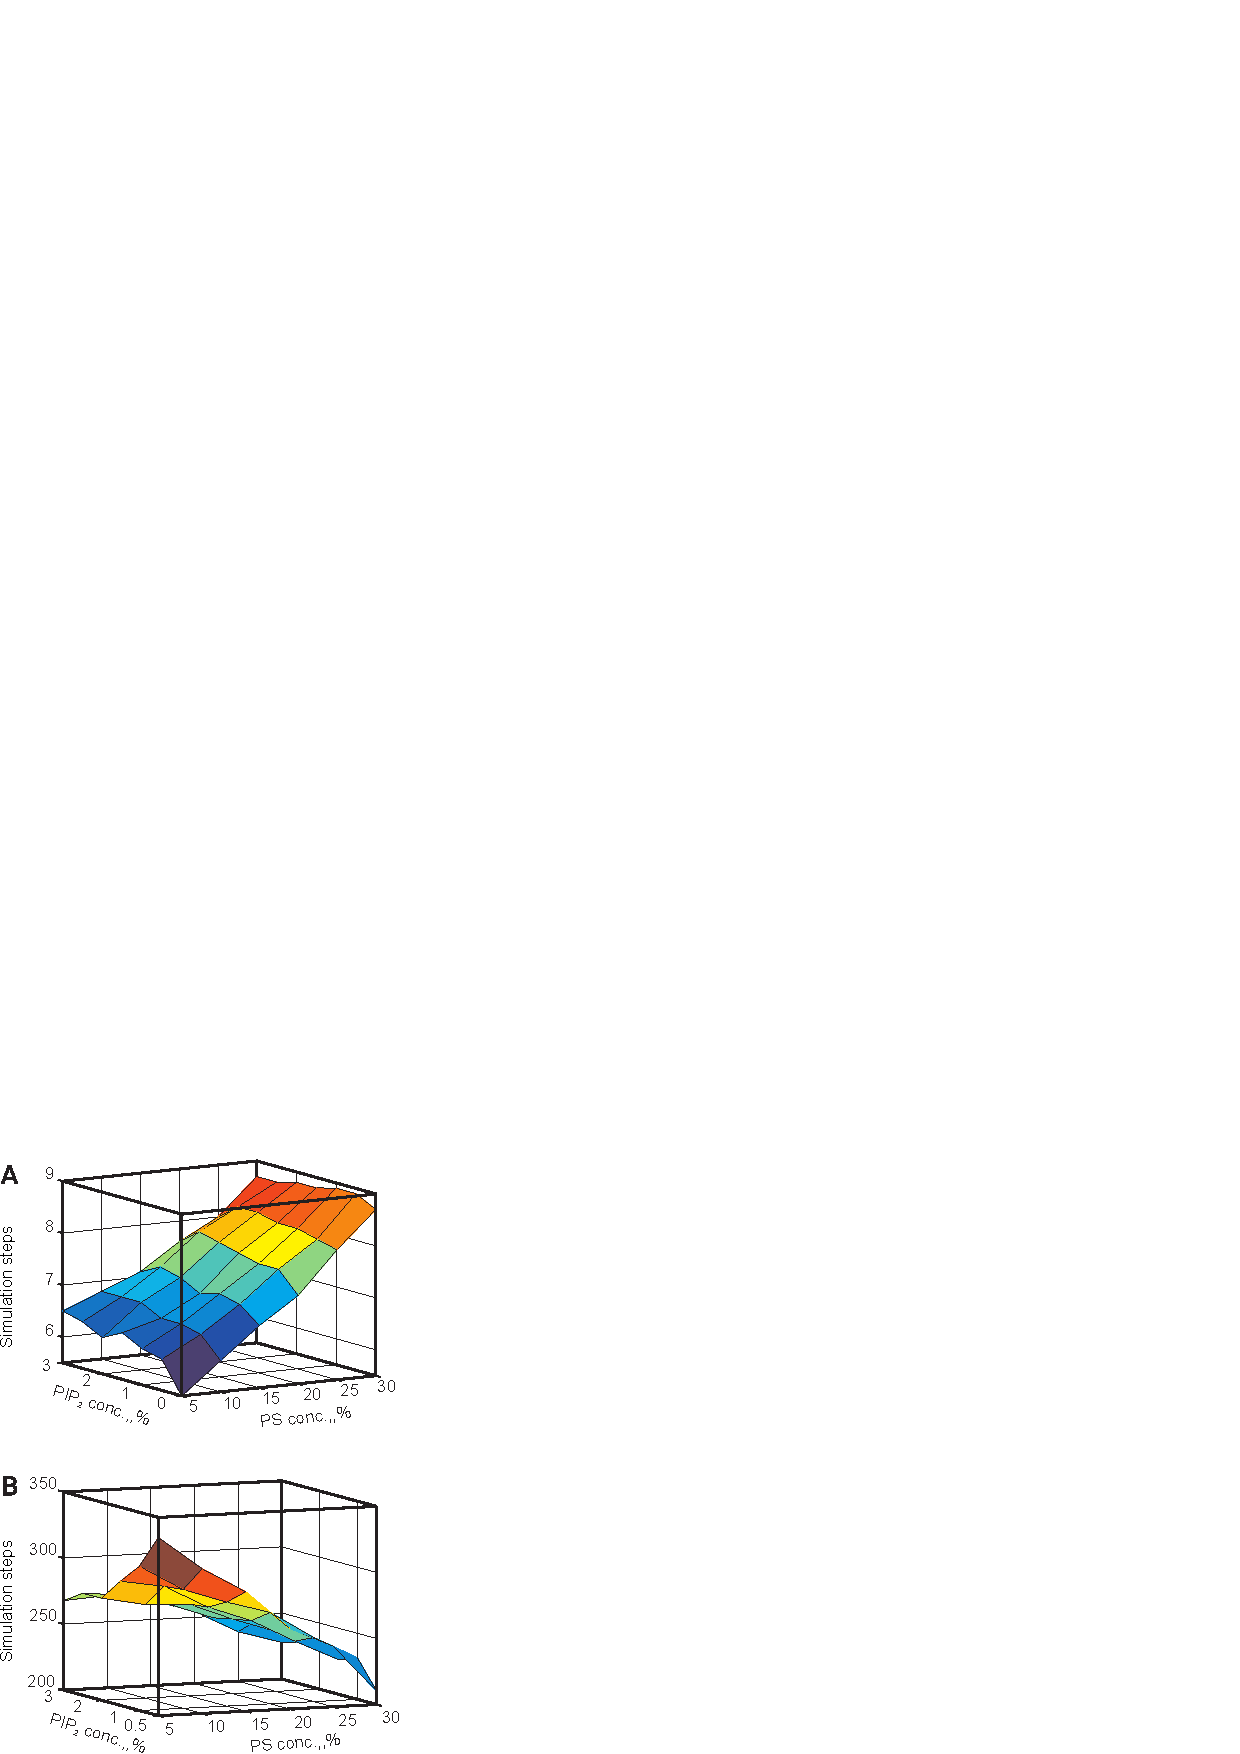
\includegraphics[scale=1.4]{../figures/lipid_association_times.pdf}
\end{center}
 \caption[Average peptide association times of PS and PIP$_2$]{Average peptide association times (from \cite{Kiselev2011}) of PS (A) and PIP$_2$ (B).}
\label{fig:lipid_association_times}
\end{figure}

Next, I measure the average association times of PS an PIP$_2$ lipids with the peptide residue (Fig. \ref{fig:lipid_association_times}). Under the assumption that $D_L$ = 1 $\mu$m$^2$/s, the association time of PS is about 5-10 simulations steps (1-2 $\mu$s), which is about 30-50 times shorter than the association time of PIP$_2$. Therefore, one can conclude that the peptide diffuses mainly together with PIP$_2$ lipids, but not with PS. These results are in agreement with the experimental data, showing that on the ternary PS/PIP$_2$/PC membrane, as opposed to the binary PS/PC membrane, the \emph{in vitro} diffusion coefficient of Lys-13 is comparable to the one of the PIP$_2$ lipids \cite{Golebiewska2006}.

Finally, I calculate average lipid probability distributions in the vicinity of the peptide. I use a square neighborhood with the center located in the position of the central peptide residue (Fig. \ref{fig:lipid_demixing_profiles}). In the absence of PIP$_2$, monovalent PS lipids strongly accumulate in between and around peptide residues. 
\begin{figure}[!ht]
%\centering
%\scalebox{1.0}[1.0]
\begin{center}
  \includegraphics{../figures/lipid_demixing_profiles.pdf}
\end{center}
 \caption[Lipid demixing profiles]{Lipid demixing caused by the peptide (from \cite{Kiselev2011}). Pseudocolor represents deviation of the local concentration of PS (A) and PIP$_2$ (B) from the expected average values indicated in the figure. (A) PIP$_2$ concentration is 0\%. (B) PS concentration is 25\%. To produce a smooth concentration field, the true values were projected from the sparse hexagonal lipid lattice onto a fine square grid and intermediate values were computed by spline interpolation. Large values corresponding to the lipid positions located directly underneath the peptide nodes (solid circles) have been removed to reveal subtle details.}
\label{fig:lipid_demixing_profiles}
\end{figure}
However, due to Debye screening, accumulation profiles do not extend further than 1 lipid node away from the peptide. It is also shown in the figure that the sequestration of PS lipids by the peptide saturates with the PS concentration. An increase of the PS concentration higher than 25\% does not significantly change its probability distribution in the vicinity of the peptide. In contrast, PIP$_2$ probability distributions in the ternary PC/PS/PIP$_2$ membrane have reversed profiles. As expected, PIP$_2$ lipids quickly accumulate in the preferable positions underneath the peptide residues. Since the repulsion between two PIP$_2$ lipids by far overcompensate the attraction to the peptide residues (see subsection \ref{interaction_energies}), the rest of PIP$_2$ lipids cannot accumulate in the peptide vicinity. In fact, free PIP$_2$ lipids are almost never found between the peptide nodes. A similar depletion effect (to a lesser extent) is also observed for the PS lipids in the ternary membrane.

The results shown in this chapter indicate that membrane lipids undergo lateral demixing and are sequestered by the peptide basic residues. However, I also measured the relative values of the lipid enrichment on the peptide, i.e. the ratio between the number of lipids found in the membrane area perturbed by the peptide and the number of lipids that would be found in the same area in the absence of the peptide. Using a symmetric hexagonal neighborhood (37 nodes) of the central peptide residue and the data presented in Fig. \ref{fig:lipid_demixing_profiles}, I obtain the following values of the relative enrichment: at the concentration of 1\% in the ternary membrane, PIP$_2$ are enriched by about $\sim$10-fold, whereas PS lipids at 35\% concentration in the binary membrane are enriched only by about 1.26. Thus, the peptide mainly sequesters PIP$_2$ lipids, but not PS. These results are in agreement with previously reported experimental data \cite{Wang2002,Gambhir2004,Golebiewska2006}.

\subsection{Peptide diffusion on the uniform membrane}

Having described the lipid demixing effect and obtained an agreement with experimental data, I then measured the peptide lateral diffusion coefficients on different (uniform) membrane compositions. In the case of the binary PC/PS membrane, Fig. \ref{fig:peptide_diffusion}, A shows that there is no systematic variation of the peptide diffusion coefficient in a broad range of PS concentrations (10-30\%). These results are in agreement with earlier data \cite{Golebiewska2006} and are not surprising, since the peptide only weakly interacts with monovalent PS lipids. However, a small reduction of the peptide diffusion coefficient from its maximal value $D_0$ to a reduced value $D'\approx0.86D_0$ is seen between 0\% and 10\% of PS. A similar weak reduction was also theoretically observed earlier \cite{Khelashvili2008}. This effect can be a consequence of the formation of a lipid shell in the vicinity of the peptide due to the rapid lipid demixing (Fig. \ref{fig:lipid_demixing_profiles}, A). The effective friction associated with the lipid shell can potentially reduce the peptide diffusion coefficient.
\begin{figure}[!ht]
%\centering
%\scalebox{1.0}[1.0]
\begin{center}
  \includegraphics[scale=1.15]{../figures/peptide_diffusion.pdf}
\end{center}
 \caption[Dependence of the peptide diffusion coefficient on the membrane composition]{Dependence of the peptide diffusion coefficient on the concentration of PS (A) and PIP$_2$ (B) (from \cite{Kiselev2011}). All simulations in B were performed with 25\% of PS; therefore, at 0\% of PIP$_2$, the peptide diffusion coefficient, $D'$, is already $<D_0$.}
\label{fig:peptide_diffusion}
\end{figure}

Fig. \ref{fig:peptide_diffusion}, B shows the dependence of the peptide diffusion coefficient on PIP$_2$ concentration. Clearly, PIP$_2$ lipids, even at a small membrane concentration, significantly reduce the peptide lateral dynamics. This behavior can potentially be explained by the following independent arguments.

First, upon the sequestration of PIP$_2$ lipids the total charge of the peptide-lipid complex becomes strongly negative (see Fig. \ref{fig:total_peptide_charge}). The diffusion of the complex in the membrane can be compared with the diffusion of a strongly negatively charged particle in the two-dimensional suspension of strongly negatively charged particles (PIP$_2$). Due to the Debye screening, Coulombic repulsion between the particles becomes a finite-radius interaction, which can be approximated by the hard-sphere potential. According to Einstein formula for a dilute solution of hard spheres:
\begin{equation}
\label{Einstein_formula}
 D^*=\frac{D'}{\eta} = \frac{D'}{1+\alpha\phi}
\end{equation}
where $D^*$ is the reduced diffusion coefficient, $\eta$ is the viscosity of the solution, and $\phi$ is the molar fraction of hard spheres. If one assumes that $\phi$ is directly proportional to PIP$_2$ membrane fraction, then it is possible to fit the simulation data of the peptide diffusion coefficient by the analytical function obtained from eq. \eqref{Einstein_formula} (see Fig. \ref{fig:peptide_diffusion}, B).

Second, Fig. \ref{fig:lipid_demixing_profiles}, B shows that the size of the PIP$_2$ lipid shell increases together with PIP$_2$ concentration. The increase of the effective friction associated with the PIP$_2$ lipid shell could also reduce the peptide diffusion according to eq. \eqref{Einstein_formula}.



